\documentclass{article}

\usepackage{graphicx}
\usepackage{tikz}
\usepackage{tikzsymbols}
\usetikzlibrary{calc,patterns,shapes.geometric}
\pagestyle{empty}
\usepackage[margin=0pt]{geometry}
\geometry{papersize={14in,12in}}

\def\centerarc[#1](#2)(#3:#4:#5){\draw[#1] ($(#2)+({#5*cos(#3)},{#5*sin(#3)})$) arc (#3:#4:#5);}

\begin{document}
	\begin{figure}
		\centering
		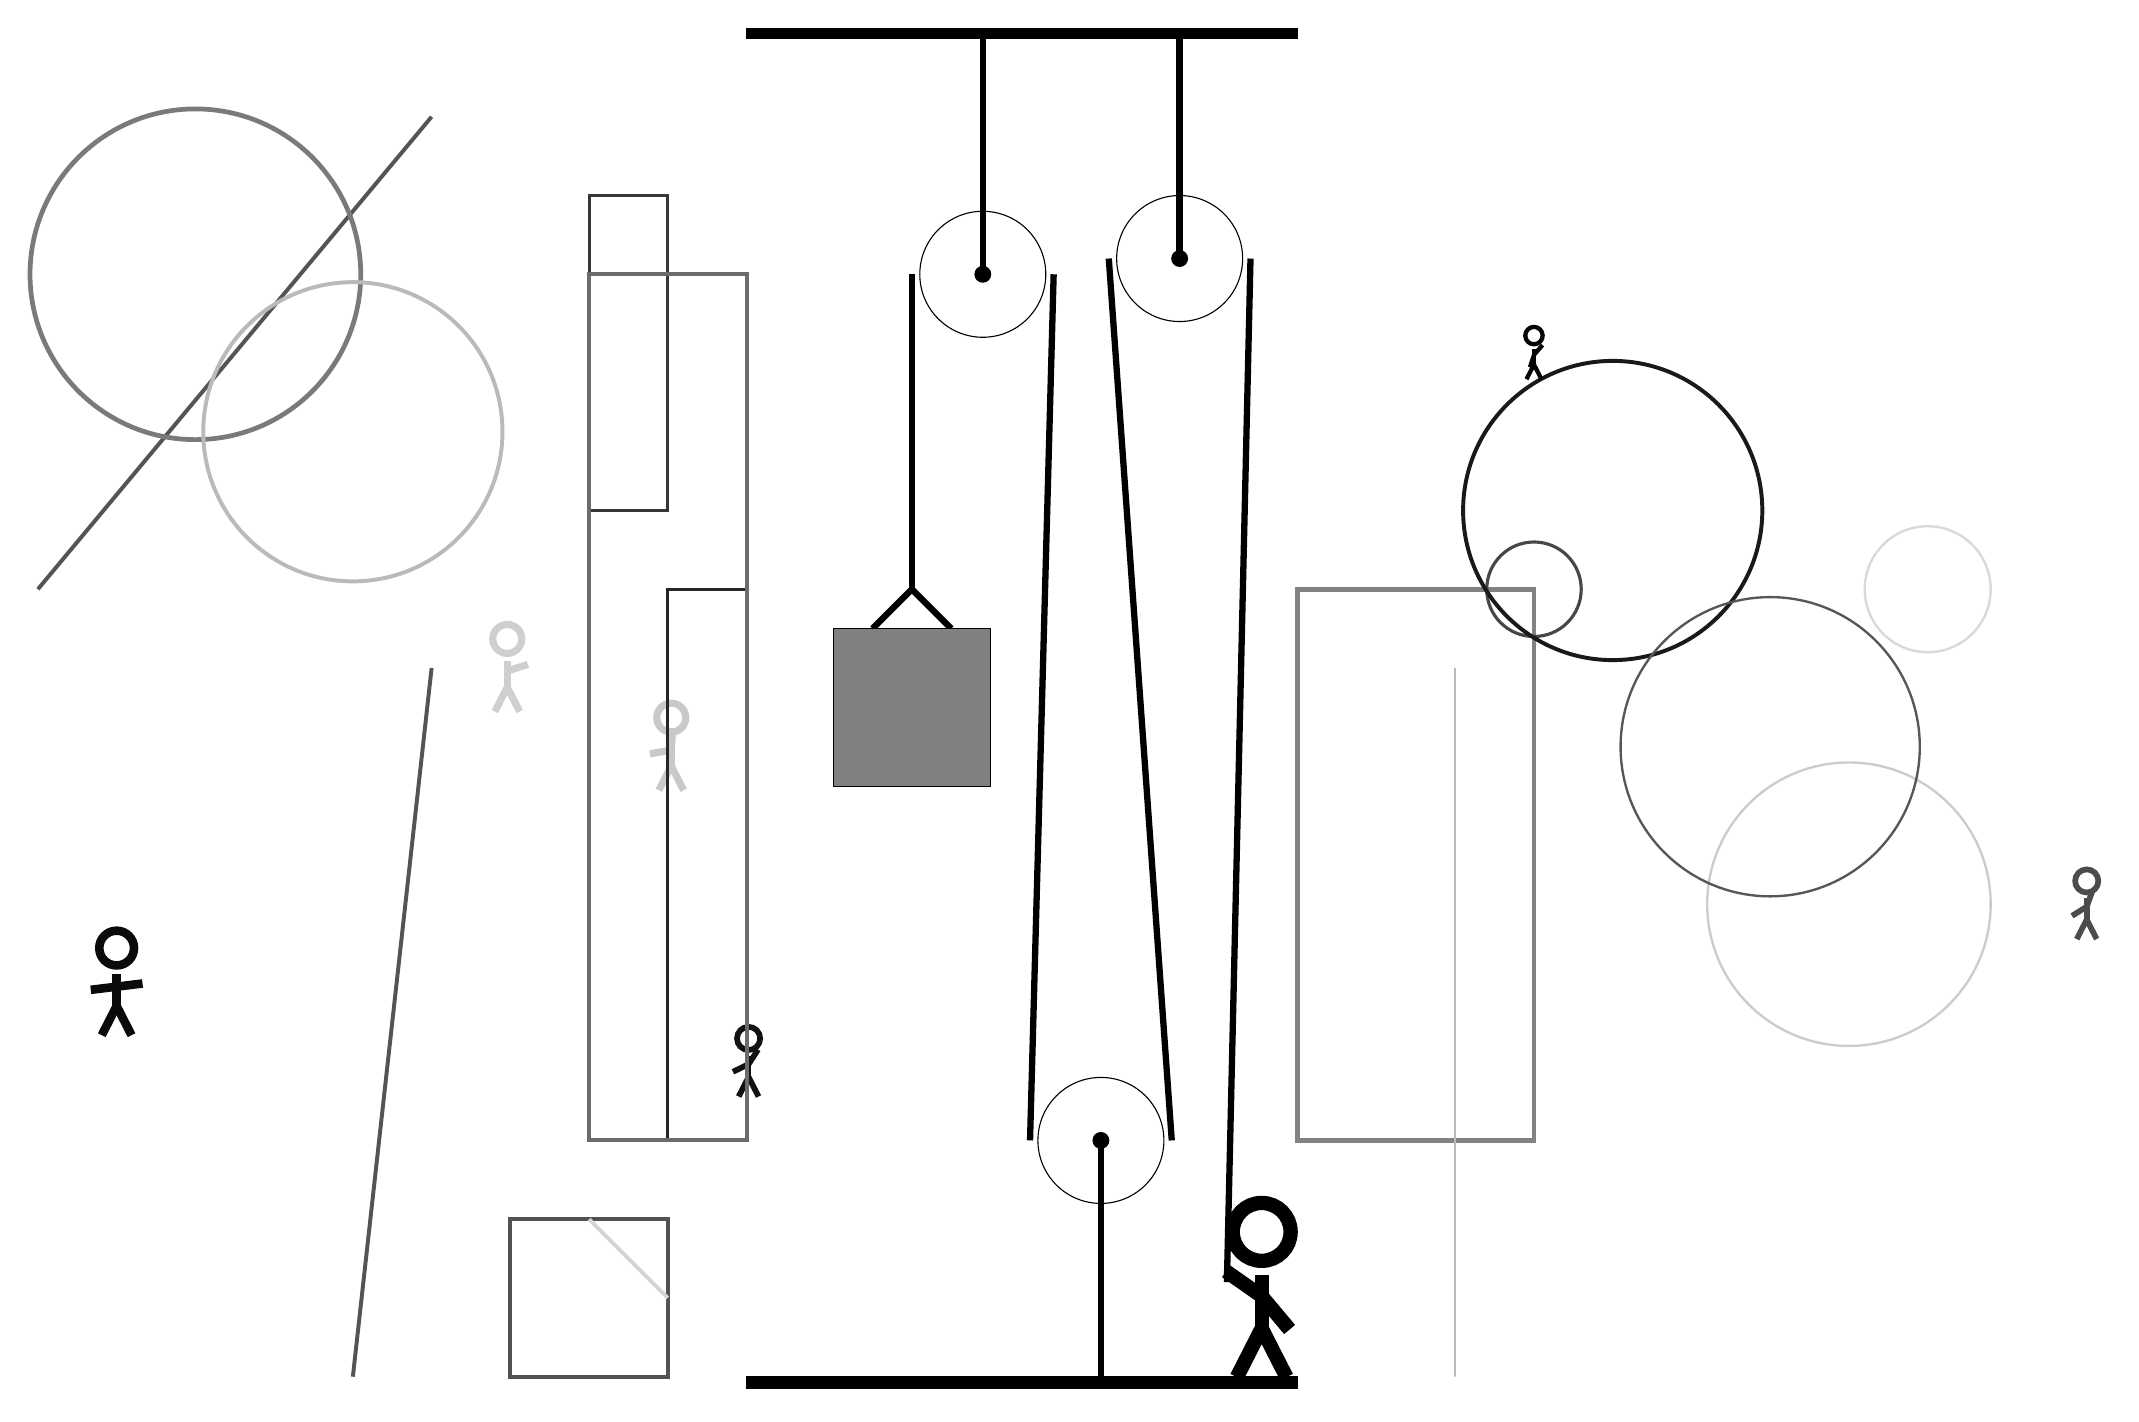
\begin{tikzpicture}
			%%%%% START %%%%%
			
			\draw[fill=black] (-2, 14) rectangle (5, 14.125);
			
			\draw (1, 11) circle (0.8);
			\draw[fill=black] (1, 11) circle (0.1);
			\draw[line width=0.8mm]  (1, 14) -- (1, 11);
			
			\draw [line width=0.3mm, color=black!15](13, 7) circle (0.8);
			
			\draw[line width=0.4mm, color=black!79] (-4, 8) rectangle (-3, 12);
			\node[line width=0.6mm, color=black!21] at (-3, 5) {\Strichmaxerl[5][11][86]};
			\draw[line width=0.5mm, color=black!68] (-3, -3) rectangle (-5, -1);
			
			\node[line width=0.7mm, color=black!96] at (-10, 2) {\Strichmaxerl[6][7][7]};
			\draw[line width=0.6mm, color=black!49] (5, 7) rectangle (8, 0);
			
			\draw[line width=0.5mm, color=black!67](-6, 13) -- (-11, 7);
			\draw [line width=0.3mm, color=black!20](12, 3) circle (1.8);
			\draw [line width=0.4mm, color=black!72](8, 7) circle (0.6);
			\draw[line width=0.4mm, color=black!85] (-2, 0) rectangle (-3, 7);
			
			\draw[line width=0.5mm, color=black!67](-6, 6) -- (-7, -3);
			
			\draw [line width=0.5mm, color=black!90](9, 8) circle (1.9);
			\draw [line width=0.6mm, color=black!52](-9, 11) circle (2.1);
			
			\draw [line width=0.5mm, color=black!27](-7, 9) circle (1.9);
			\node[line width=0.3mm, color=black!70] at (15, 3) {\Strichmaxerl[4][32][70]};
			\node[line width=0.2mm, color=black!93] at (-2, 1) {\Strichmaxerl[4][26][57]};
			
			\draw [line width=0.3mm, color=black!66](11, 5) circle (1.9);
			
			\draw[line width=0.2mm, color=black!27] (7, -3) rectangle (7, 6);
			\draw[line width=0.5mm, color=black!17](-3, -2) -- (-4, -1);
			\draw[line width=0.5mm, color=black!58] (-2, 0) rectangle (-4, 11);
			\node[line width=0.5mm, color=black!98] at (8, 10) {\Strichmaxerl[3][72][49]};
			\node[line width=0.3mm, color=black!19] at (-5, 6) {\Strichmaxerl[5][90][18]};
			
			
			\draw[fill=white](2.5, 0) circle (0.8);
			\draw[fill=black] (2.5, 0) circle (0.1);
			\draw[line width=0.8mm]  (2.5, -3) -- (2.5, 0);
			
			\draw[fill=white](3.5, 11.2) circle (0.8);
			\draw[fill=black] (3.5, 11.2) circle (0.1);
			\draw[line width=0.8mm] (3.5, 14) -- (3.5, 11.2);
			
			\draw[line width=0.8mm] (-0.4, 6.5) -- (0.1, 7.0) -- (0.6, 6.5);
			\draw[fill=black!50] (-0.9, 6.5) rectangle (1.1, 4.5);
			
			\draw[line width=0.8mm] (0.1, 11) -- (0.1, 7.0);
			\centerarc[line width=0.8mm](1, 11)(0:180:0.9);
			\draw[line width=0.8mm](1.9, 11) -- (1.6, 0);
			\centerarc[line width=0.8mm](2.5, 0)(180:360:0.9);
			\draw[line width=0.8mm](3.4, 0) -- (2.6, 11.2);
			\centerarc[line width=0.8mm](3.5, 11.2)(0:180:0.9);
			\draw[line width=0.8mm](4.4, 11.2) -- (4.1, -1.8);
			
			\node at (4.5, -1.9) {\Strichmaxerl[10][-35][-50]};
			
			\draw[fill=black] (-2, -3) rectangle (5, -3.15);
			
			%%%%% END %%%%%
		\end{tikzpicture}
	\end{figure}	
\end{document}